\documentclass[
  de, % or de
  inputenc=utf8,
  %aspectratio=169,
]{tuhhslides}

% use flat boxes
\setbeamertemplate{blocks}[flat]


% setup title, author and institute
\title[Reverse Engineering eines Kaffeevollautomaten]{Reverse Engineering eines\\Kaffeevollautomaten}
\author[]{\speaker{Niklas Joachim Eberhard Kr\"uger}}
%%% as Student do not use any Institute tag or use the following
\institute{InstSchoolOfEEIT}
%%%
%%% as Staff you can use your Institute see tuhhlangnames.def
%\institute{InstTelematics}
%\institute{InstSmartPort}
%%%
\subject{Abschlussvortrag, Bachelorarbeit, Meyer}
\date{06.03.2019}

%%
\usepackage{listings}
\usepackage{savesym}
\savesymbol{checkmark}
\usepackage{dingbat} % for \carriagereturn
\usepackage[export]{adjustbox} % frame around highlighted image area

% animated and user defined tikzpictues
\usepackage{tikz}
\usetikzlibrary{matrix}
\tikzset{
  matrixstyle/.style={
    matrix of nodes,
    nodes in empty cells,
    column sep      = 0.1cm,
    row sep         = -\pgflinewidth,
    nodes={%
      inner sep=0mm,outer sep=0pt,
      minimum size=5mm,
      text height=\ht\strutbox,text depth=\dp\strutbox,
      %draw
    },%
  },
  changed/.style={}, % siehe unten: \only<...
  blanked/.style={}, % siehe unten: \only<...
  final/.style={},   % siehe unten: \only<...
  %
  % Animation in dem tikz picture Objekt
  invisible/.style={opacity=0},
  visible on/.style={alt={#1{}{invisible}}},
  alt/.code args={<#1>#2#3}{%
    \alt<#1>{\pgfkeysalso{#2}}{\pgfkeysalso{#3}} % \pgfkeysalso doesn't change the path
  },
}

%% enable section page
\AtBeginSection{%
  \frame[plain,noframenumbering]{\sectionpage}
}

\begin{document}

%% title page
\begin{frame}[plain,noframenumbering]
    \titlepage
\end{frame}

%% table of content
\begin{frame}
    \frametitle{\"Ubersicht}
    \tableofcontents
\end{frame}



\section{Aufbau und Kommunikation}
\begin{frame}{Zugriff direkt oder über die UART Schnittstelle}
  Direkte Speicherabfrage:
  \begin{itemize}
    \item Aktives Eingreifen verursacht Kurzschlüsse im Betrieb
  \end{itemize}
  \vspace{1cm}
  Serielle UART Schnittstelle:
  \begin{itemize}
    \item Vorteil: RAM und EEPROM Abfrage im laufenden Betrieb
    \item Nachteil: Zeitintensiv\\\hspace{1.5cm}$\Rightarrow$ kein konsistenter Speicherauszug
    \item Nachteil: Hemmt das interne Bussystem
  \end{itemize}
\end{frame}

\begin{frame}
  \begin{center}
    \begin{tikzpicture}
      \node (img1) {\includegraphics[scale=0.21]{Material/Jura-Impressa-S9-small.png}};
    \end{tikzpicture}
  \end{center}
\end{frame}
\begin{frame}{Probleme bei der seriellen Kommunikation}
  \begin{itemize}
    \item Initialisierung benötigt mehrere Anläufe
    \item Kaum reproduzierbares Fehlverhalten beim direkten Zugriff auf die Gerätedatei
    \item Initialisierte Umgebung ließ sich nicht über\\\texttt{stty -F /dev/ttyACM0} nachbauen
    \item $\Rightarrow$ \textit{libserial}-Library
  \end{itemize}
\end{frame}



\section{Speicher}
\begin{frame}{EEPROM}
  \begin{figure}
    \begin{center}
      \hspace*{-1cm}
      \includegraphics[scale=0.46]{Material/Speicher-Schema-Jura-EEPROM}
    \end{center}
  \end{figure}
\end{frame}

\begin{frame}{RAM}
  \begin{figure}
    \begin{center}
      \hspace*{-1cm}
      \includegraphics[scale=0.46]{Material/Speicher-Schema-Jura-Ram}
    \end{center}
  \end{figure}
\end{frame}



\section{Vorgehen}
\begin{frame}{Standardverfahren}
  \begin{figure}
    \begin{center}
      \hspace*{-1cm}
      \includegraphics[scale=0.54]{Material/workflow}
    \end{center}
  \end{figure}
\end{frame}

\begin{frame}{Weitere Ansätze}
  \begin{itemize}
    \item Regelmäßige Unregelmäßigkeiten im RAM ausgeblendet
    \item Zähler im EEPROM verändert
    \item ASCII Tabelle für Zeichensatz des Displays angewendet
  \end{itemize}
\end{frame}

\begin{frame}{Implementierung in C++}
  \begin{figure}
    \begin{center}
      \hspace*{-0.9cm}
      \includegraphics[scale=0.65]{Material/class-structure}
    \end{center}
  \end{figure}
\end{frame}



\section{Ergebnisse}
\begin{frame}{EEPROM}
  \vspace*{-0.5cm}
  \begin{center}
    \begin{tikzpicture}
      \only<1-5>{
        \node (img1) {\includegraphics[scale=0.165]{Material/Speicher-Auswertung-EEPROM}};
      }
      \only<2>{
        \node (img2) at (img1) {
          \colorbox{white}{
%             \vspace*{-3cm}
             \hspace*{-1.2cm}
            \includegraphics[scale=1.2,trim={0 42.4cm 38cm 0},clip,fbox]{Material/Speicher-Auswertung-EEPROM}
          }
        };
      }
      \only<3>{
        \node (img3) at (img1) {
          \colorbox{white}{
%             \vspace*{-3cm}
             \hspace*{-1.2cm}
            \includegraphics[scale=1.2,trim={0 39cm 38cm 6.5cm},clip,fbox]{Material/Speicher-Auswertung-EEPROM}
          }
        };
      }
      \only<4>{
        \node (img4) at (img1) {
          \colorbox{white}{
%             \vspace*{-3cm}
             \hspace*{-1.2cm}
            \includegraphics[scale=1.2,trim={0 21.5cm 38cm 22.9cm},clip,fbox]{Material/Speicher-Auswertung-EEPROM}
          }
        };
      }
      \only<5>{
        \node (img5) at (img1) {
          \colorbox{white}{
%             \vspace*{-3cm}
             \hspace*{-1.2cm}
            \includegraphics[scale=1.2,trim={0 12.2cm 38cm 32.05cm},clip,fbox]{Material/Speicher-Auswertung-EEPROM}
          }
        };
      }
    \end{tikzpicture}
  \end{center}
\end{frame}
\begin{frame}{RAM}
  \vspace*{-1.2cm}
  \begin{center}
    \begin{tikzpicture}
      \only<1-4>{
        \node (img1) {\includegraphics[scale=0.365]{Material/Speicher-Auswertung-RAM}};
      }
      \only<2>{
        \node (img2) at (img1) {
          \colorbox{white}{
            \includegraphics[scale=1.6,trim={0 19cm 0 0},clip,fbox]{Material/Speicher-Auswertung-RAM}
          }
        };
      }
      \only<3>{
        \node (img3) at (img1) {
          \colorbox{white}{
            \includegraphics[scale=1.6,trim={0 10.5cm 0 9.05cm},clip,fbox]{Material/Speicher-Auswertung-RAM}
          }
        };
      }
      \only<4>{
        \node (img4) at (img1) {
          \colorbox{white}{
            \includegraphics[scale=1.6,trim={0 0 0 21.5cm},clip,fbox]{Material/Speicher-Auswertung-RAM}
          }
        };
      }
    \end{tikzpicture}
  \end{center}
\end{frame}

\section{Terminologie "`Reverse Engineering"'}
\begin{frame}{Begriffe}
  \begin{columns}
    \begin{column}{0.37\textwidth}
      \begin{itemize}
        \item Forward Engineering\vspace{0.25cm}
        \item Reverse Engineering
      \end{itemize}
    \end{column}
    \begin{column}{0.33\textwidth}
      \begin{itemize}
        \item Redocumentation\vspace{0.25cm}
        \item Design Recovery
      \end{itemize}
    \end{column}
    \begin{column}{0.3\textwidth}
      \begin{itemize}
        \item Restructuring\vspace{0.25cm}
        \item Reengineering
      \end{itemize}
    \end{column}
  \end{columns}
  \begin{center}
    \resizebox{11.5cm}{6cm}{%
      % Graphic for TeX using PGF
% Title: /home/niklas/Desktop/JuraCoffeeThesis/Abschlussvortrag/Material/abstraction-levels-software-engineering.dia
% Creator: Dia v0.97+git
% CreationDate: Fri Mar  1 13:40:47 2019
% For: niklas
% \usepackage{tikz}
% The following commands are not supported in PSTricks at present
% We define them conditionally, so when they are implemented,
% this pgf file will use them.
\ifx\du\undefined
  \newlength{\du}
\fi
\setlength{\du}{15\unitlength}
\begin{tikzpicture}[even odd rule]
\pgftransformxscale{1.000000}
\pgftransformyscale{-1.000000}
\definecolor{dialinecolor}{rgb}{0.000000, 0.000000, 0.000000}
\pgfsetstrokecolor{dialinecolor}
\pgfsetstrokeopacity{1.000000}
\definecolor{diafillcolor}{rgb}{1.000000, 1.000000, 1.000000}
\pgfsetfillcolor{diafillcolor}
\pgfsetfillopacity{1.000000}
\pgfsetlinewidth{0.200000\du}
\pgfsetdash{}{0pt}
\pgfsetmiterjoin
{\pgfsetcornersarced{\pgfpoint{0.000000\du}{0.000000\du}}\definecolor{diafillcolor}{rgb}{1.000000, 1.000000, 1.000000}
\pgfsetfillcolor{diafillcolor}
\pgfsetfillopacity{1.000000}
\fill (28.050000\du,13.000000\du)--(28.050000\du,15.800000\du)--(32.055000\du,15.800000\du)--(32.055000\du,13.000000\du)--cycle;
}{\pgfsetcornersarced{\pgfpoint{0.000000\du}{0.000000\du}}\definecolor{dialinecolor}{rgb}{1.000000, 1.000000, 1.000000}
\pgfsetstrokecolor{dialinecolor}
\pgfsetstrokeopacity{1.000000}
\draw (28.050000\du,13.000000\du)--(28.050000\du,15.800000\du)--(32.055000\du,15.800000\du)--(32.055000\du,13.000000\du)--cycle;
}% setfont left to latex
\definecolor{dialinecolor}{rgb}{0.000000, 0.000000, 0.000000}
\pgfsetstrokecolor{dialinecolor}
\pgfsetstrokeopacity{1.000000}
\definecolor{diafillcolor}{rgb}{0.000000, 0.000000, 0.000000}
\pgfsetfillcolor{diafillcolor}
\pgfsetfillopacity{1.000000}
\node[anchor=base,inner sep=0pt, outer sep=0pt,color=dialinecolor] at (30.052500\du,14.195000\du){Design};
% setfont left to latex
\definecolor{dialinecolor}{rgb}{0.000000, 0.000000, 0.000000}
\pgfsetstrokecolor{dialinecolor}
\pgfsetstrokeopacity{1.000000}
\definecolor{diafillcolor}{rgb}{0.000000, 0.000000, 0.000000}
\pgfsetfillcolor{diafillcolor}
\pgfsetfillopacity{1.000000}
\node[anchor=base,inner sep=0pt, outer sep=0pt,color=dialinecolor] at (30.052500\du,14.995000\du){recovery};
\pgfsetlinewidth{0.200000\du}
\pgfsetdash{{\pgflinewidth}{0.200000\du}}{0cm}
\pgfsetmiterjoin
{\pgfsetcornersarced{\pgfpoint{0.000000\du}{0.000000\du}}\definecolor{diafillcolor}{rgb}{1.000000, 1.000000, 1.000000}
\pgfsetfillcolor{diafillcolor}
\pgfsetfillopacity{1.000000}
\fill (33.000000\du,24.400000\du)--(33.000000\du,26.400000\du)--(38.522500\du,26.400000\du)--(38.522500\du,24.400000\du)--cycle;
}{\pgfsetcornersarced{\pgfpoint{0.000000\du}{0.000000\du}}\definecolor{dialinecolor}{rgb}{1.000000, 1.000000, 1.000000}
\pgfsetstrokecolor{dialinecolor}
\pgfsetstrokeopacity{1.000000}
\draw (33.000000\du,24.400000\du)--(33.000000\du,26.400000\du)--(38.522500\du,26.400000\du)--(38.522500\du,24.400000\du)--cycle;
}% setfont left to latex
\definecolor{dialinecolor}{rgb}{0.000000, 0.000000, 0.000000}
\pgfsetstrokecolor{dialinecolor}
\pgfsetstrokeopacity{1.000000}
\definecolor{diafillcolor}{rgb}{0.000000, 0.000000, 0.000000}
\pgfsetfillcolor{diafillcolor}
\pgfsetfillopacity{1.000000}
\node[anchor=base,inner sep=0pt, outer sep=0pt,color=dialinecolor] at (35.761250\du,25.595000\du){Restructuring};
\pgfsetlinewidth{0.200000\du}
\pgfsetdash{{\pgflinewidth}{0.200000\du}}{0cm}
\pgfsetmiterjoin
{\pgfsetcornersarced{\pgfpoint{0.000000\du}{0.000000\du}}\definecolor{diafillcolor}{rgb}{1.000000, 1.000000, 1.000000}
\pgfsetfillcolor{diafillcolor}
\pgfsetfillopacity{1.000000}
\fill (19.000000\du,24.400000\du)--(19.000000\du,26.400000\du)--(24.522500\du,26.400000\du)--(24.522500\du,24.400000\du)--cycle;
}{\pgfsetcornersarced{\pgfpoint{0.000000\du}{0.000000\du}}\definecolor{dialinecolor}{rgb}{1.000000, 1.000000, 1.000000}
\pgfsetstrokecolor{dialinecolor}
\pgfsetstrokeopacity{1.000000}
\draw (19.000000\du,24.400000\du)--(19.000000\du,26.400000\du)--(24.522500\du,26.400000\du)--(24.522500\du,24.400000\du)--cycle;
}% setfont left to latex
\definecolor{dialinecolor}{rgb}{0.000000, 0.000000, 0.000000}
\pgfsetstrokecolor{dialinecolor}
\pgfsetstrokeopacity{1.000000}
\definecolor{diafillcolor}{rgb}{0.000000, 0.000000, 0.000000}
\pgfsetfillcolor{diafillcolor}
\pgfsetfillopacity{1.000000}
\node[anchor=base,inner sep=0pt, outer sep=0pt,color=dialinecolor] at (21.761250\du,25.595000\du){Restructuring};
\pgfsetlinewidth{0.200000\du}
\pgfsetdash{{\pgflinewidth}{0.200000\du}}{0cm}
\pgfsetmiterjoin
{\pgfsetcornersarced{\pgfpoint{0.000000\du}{0.000000\du}}\definecolor{diafillcolor}{rgb}{1.000000, 1.000000, 1.000000}
\pgfsetfillcolor{diafillcolor}
\pgfsetfillopacity{1.000000}
\fill (5.000000\du,24.400000\du)--(5.000000\du,26.400000\du)--(10.522500\du,26.400000\du)--(10.522500\du,24.400000\du)--cycle;
}{\pgfsetcornersarced{\pgfpoint{0.000000\du}{0.000000\du}}\definecolor{dialinecolor}{rgb}{1.000000, 1.000000, 1.000000}
\pgfsetstrokecolor{dialinecolor}
\pgfsetstrokeopacity{1.000000}
\draw (5.000000\du,24.400000\du)--(5.000000\du,26.400000\du)--(10.522500\du,26.400000\du)--(10.522500\du,24.400000\du)--cycle;
}% setfont left to latex
\definecolor{dialinecolor}{rgb}{0.000000, 0.000000, 0.000000}
\pgfsetstrokecolor{dialinecolor}
\pgfsetstrokeopacity{1.000000}
\definecolor{diafillcolor}{rgb}{0.000000, 0.000000, 0.000000}
\pgfsetfillcolor{diafillcolor}
\pgfsetfillopacity{1.000000}
\node[anchor=base,inner sep=0pt, outer sep=0pt,color=dialinecolor] at (7.761250\du,25.595000\du){Restructuring};
\pgfsetlinewidth{0.200000\du}
\pgfsetdash{{\pgflinewidth}{0.200000\du}}{0cm}
\pgfsetmiterjoin
{\pgfsetcornersarced{\pgfpoint{0.000000\du}{0.000000\du}}\definecolor{diafillcolor}{rgb}{1.000000, 1.000000, 1.000000}
\pgfsetfillcolor{diafillcolor}
\pgfsetfillopacity{1.000000}
\fill (31.613750\du,3.041389\du)--(31.613750\du,5.158611\du)--(39.386250\du,5.158611\du)--(39.386250\du,3.041389\du)--cycle;
}{\pgfsetcornersarced{\pgfpoint{0.000000\du}{0.000000\du}}\definecolor{dialinecolor}{rgb}{1.000000, 1.000000, 1.000000}
\pgfsetstrokecolor{dialinecolor}
\pgfsetstrokeopacity{1.000000}
\draw (31.613750\du,3.041389\du)--(31.613750\du,5.158611\du)--(39.386250\du,5.158611\du)--(39.386250\du,3.041389\du)--cycle;
}% setfont left to latex
\definecolor{dialinecolor}{rgb}{0.000000, 0.000000, 0.000000}
\pgfsetstrokecolor{dialinecolor}
\pgfsetstrokeopacity{1.000000}
\definecolor{diafillcolor}{rgb}{0.000000, 0.000000, 0.000000}
\pgfsetfillcolor{diafillcolor}
\pgfsetfillopacity{1.000000}
\node[anchor=base,inner sep=0pt, outer sep=0pt,color=dialinecolor] at (35.500000\du,4.323889\du){\textbf{{\Large Implementation}}};
\pgfsetlinewidth{0.200000\du}
\pgfsetdash{{\pgflinewidth}{0.200000\du}}{0cm}
\pgfsetmiterjoin
{\pgfsetcornersarced{\pgfpoint{0.000000\du}{0.000000\du}}\definecolor{diafillcolor}{rgb}{1.000000, 1.000000, 1.000000}
\pgfsetfillcolor{diafillcolor}
\pgfsetfillopacity{1.000000}
\fill (18.000000\du,3.041389\du)--(18.000000\du,5.158611\du)--(25.000000\du,5.158611\du)--(25.000000\du,3.041389\du)--cycle;
}{\pgfsetcornersarced{\pgfpoint{0.000000\du}{0.000000\du}}\definecolor{dialinecolor}{rgb}{1.000000, 1.000000, 1.000000}
\pgfsetstrokecolor{dialinecolor}
\pgfsetstrokeopacity{1.000000}
\draw (18.000000\du,3.041389\du)--(18.000000\du,5.158611\du)--(25.000000\du,5.158611\du)--(25.000000\du,3.041389\du)--cycle;
}% setfont left to latex
\definecolor{dialinecolor}{rgb}{0.000000, 0.000000, 0.000000}
\pgfsetstrokecolor{dialinecolor}
\pgfsetstrokeopacity{1.000000}
\definecolor{diafillcolor}{rgb}{0.000000, 0.000000, 0.000000}
\pgfsetfillcolor{diafillcolor}
\pgfsetfillopacity{1.000000}
\node[anchor=base,inner sep=0pt, outer sep=0pt,color=dialinecolor] at (21.500000\du,4.323889\du){\textbf{{\Large Design}}};
\pgfsetlinewidth{0.200000\du}
\pgfsetdash{{\pgflinewidth}{0.200000\du}}{0cm}
\pgfsetmiterjoin
{\pgfsetcornersarced{\pgfpoint{0.000000\du}{0.000000\du}}\definecolor{diafillcolor}{rgb}{1.000000, 1.000000, 1.000000}
\pgfsetfillcolor{diafillcolor}
\pgfsetfillopacity{1.000000}
\fill (4.000000\du,3.041389\du)--(4.000000\du,5.158611\du)--(11.000000\du,5.158611\du)--(11.000000\du,3.041389\du)--cycle;
}{\pgfsetcornersarced{\pgfpoint{0.000000\du}{0.000000\du}}\definecolor{dialinecolor}{rgb}{1.000000, 1.000000, 1.000000}
\pgfsetstrokecolor{dialinecolor}
\pgfsetstrokeopacity{1.000000}
\draw (4.000000\du,3.041389\du)--(4.000000\du,5.158611\du)--(11.000000\du,5.158611\du)--(11.000000\du,3.041389\du)--cycle;
}% setfont left to latex
\definecolor{dialinecolor}{rgb}{0.000000, 0.000000, 0.000000}
\pgfsetstrokecolor{dialinecolor}
\pgfsetstrokeopacity{1.000000}
\definecolor{diafillcolor}{rgb}{0.000000, 0.000000, 0.000000}
\pgfsetfillcolor{diafillcolor}
\pgfsetfillopacity{1.000000}
\node[anchor=base,inner sep=0pt, outer sep=0pt,color=dialinecolor] at (7.500000\du,4.323889\du){\textbf{{\Large Requirements}}};
\pgfsetlinewidth{0.200000\du}
\pgfsetdash{}{0pt}
\pgfsetmiterjoin
{\pgfsetcornersarced{\pgfpoint{0.000000\du}{0.000000\du}}\definecolor{diafillcolor}{rgb}{1.000000, 1.000000, 1.000000}
\pgfsetfillcolor{diafillcolor}
\pgfsetfillopacity{1.000000}
\fill (25.578300\du,20.000000\du)--(25.578300\du,22.000000\du)--(31.423300\du,22.000000\du)--(31.423300\du,20.000000\du)--cycle;
}{\pgfsetcornersarced{\pgfpoint{0.000000\du}{0.000000\du}}\definecolor{dialinecolor}{rgb}{1.000000, 1.000000, 1.000000}
\pgfsetstrokecolor{dialinecolor}
\pgfsetstrokeopacity{1.000000}
\draw (25.578300\du,20.000000\du)--(25.578300\du,22.000000\du)--(31.423300\du,22.000000\du)--(31.423300\du,20.000000\du)--cycle;
}% setfont left to latex
\definecolor{dialinecolor}{rgb}{0.000000, 0.000000, 0.000000}
\pgfsetstrokecolor{dialinecolor}
\pgfsetstrokeopacity{1.000000}
\definecolor{diafillcolor}{rgb}{0.000000, 0.000000, 0.000000}
\pgfsetfillcolor{diafillcolor}
\pgfsetfillopacity{1.000000}
\node[anchor=base,inner sep=0pt, outer sep=0pt,color=dialinecolor] at (28.500800\du,21.195000\du){Reengineering};
\pgfsetlinewidth{0.200000\du}
\pgfsetdash{}{0pt}
\pgfsetmiterjoin
{\pgfsetcornersarced{\pgfpoint{0.000000\du}{0.000000\du}}\definecolor{diafillcolor}{rgb}{1.000000, 1.000000, 1.000000}
\pgfsetfillcolor{diafillcolor}
\pgfsetfillopacity{1.000000}
\fill (11.768700\du,20.000000\du)--(11.768700\du,22.000000\du)--(17.613700\du,22.000000\du)--(17.613700\du,20.000000\du)--cycle;
}{\pgfsetcornersarced{\pgfpoint{0.000000\du}{0.000000\du}}\definecolor{dialinecolor}{rgb}{1.000000, 1.000000, 1.000000}
\pgfsetstrokecolor{dialinecolor}
\pgfsetstrokeopacity{1.000000}
\draw (11.768700\du,20.000000\du)--(11.768700\du,22.000000\du)--(17.613700\du,22.000000\du)--(17.613700\du,20.000000\du)--cycle;
}% setfont left to latex
\definecolor{dialinecolor}{rgb}{0.000000, 0.000000, 0.000000}
\pgfsetstrokecolor{dialinecolor}
\pgfsetstrokeopacity{1.000000}
\definecolor{diafillcolor}{rgb}{0.000000, 0.000000, 0.000000}
\pgfsetfillcolor{diafillcolor}
\pgfsetfillopacity{1.000000}
\node[anchor=base,inner sep=0pt, outer sep=0pt,color=dialinecolor] at (14.691200\du,21.195000\du){Reengineering};
\pgfsetlinewidth{0.200000\du}
\pgfsetdash{}{0pt}
\pgfsetmiterjoin
{\pgfsetcornersarced{\pgfpoint{0.000000\du}{0.000000\du}}\definecolor{diafillcolor}{rgb}{1.000000, 1.000000, 1.000000}
\pgfsetfillcolor{diafillcolor}
\pgfsetfillopacity{1.000000}
\fill (4.000000\du,5.000000\du)--(4.000000\du,23.000000\du)--(11.000000\du,23.000000\du)--(11.000000\du,5.000000\du)--cycle;
}{\pgfsetcornersarced{\pgfpoint{0.000000\du}{0.000000\du}}\definecolor{dialinecolor}{rgb}{0.000000, 0.000000, 0.000000}
\pgfsetstrokecolor{dialinecolor}
\pgfsetstrokeopacity{1.000000}
\draw (4.000000\du,5.000000\du)--(4.000000\du,23.000000\du)--(11.000000\du,23.000000\du)--(11.000000\du,5.000000\du)--cycle;
}% setfont left to latex
\definecolor{dialinecolor}{rgb}{0.000000, 0.000000, 0.000000}
\pgfsetstrokecolor{dialinecolor}
\pgfsetstrokeopacity{1.000000}
\definecolor{diafillcolor}{rgb}{0.000000, 0.000000, 0.000000}
\pgfsetfillcolor{diafillcolor}
\pgfsetfillopacity{1.000000}
\node[anchor=base,inner sep=0pt, outer sep=0pt,color=dialinecolor] at (7.500000\du,14.195000\du){};
\pgfsetlinewidth{0.200000\du}
\pgfsetdash{}{0pt}
\pgfsetmiterjoin
{\pgfsetcornersarced{\pgfpoint{0.000000\du}{0.000000\du}}\definecolor{diafillcolor}{rgb}{1.000000, 1.000000, 1.000000}
\pgfsetfillcolor{diafillcolor}
\pgfsetfillopacity{1.000000}
\fill (18.000000\du,5.000000\du)--(18.000000\du,23.000000\du)--(25.000000\du,23.000000\du)--(25.000000\du,5.000000\du)--cycle;
}{\pgfsetcornersarced{\pgfpoint{0.000000\du}{0.000000\du}}\definecolor{dialinecolor}{rgb}{0.000000, 0.000000, 0.000000}
\pgfsetstrokecolor{dialinecolor}
\pgfsetstrokeopacity{1.000000}
\draw (18.000000\du,5.000000\du)--(18.000000\du,23.000000\du)--(25.000000\du,23.000000\du)--(25.000000\du,5.000000\du)--cycle;
}% setfont left to latex
\definecolor{dialinecolor}{rgb}{0.000000, 0.000000, 0.000000}
\pgfsetstrokecolor{dialinecolor}
\pgfsetstrokeopacity{1.000000}
\definecolor{diafillcolor}{rgb}{0.000000, 0.000000, 0.000000}
\pgfsetfillcolor{diafillcolor}
\pgfsetfillopacity{1.000000}
\node[anchor=base,inner sep=0pt, outer sep=0pt,color=dialinecolor] at (21.500000\du,14.195000\du){};
\pgfsetlinewidth{0.200000\du}
\pgfsetdash{}{0pt}
\pgfsetmiterjoin
{\pgfsetcornersarced{\pgfpoint{0.000000\du}{0.000000\du}}\definecolor{diafillcolor}{rgb}{1.000000, 1.000000, 1.000000}
\pgfsetfillcolor{diafillcolor}
\pgfsetfillopacity{1.000000}
\fill (32.000000\du,5.000000\du)--(32.000000\du,23.000000\du)--(39.000000\du,23.000000\du)--(39.000000\du,5.000000\du)--cycle;
}{\pgfsetcornersarced{\pgfpoint{0.000000\du}{0.000000\du}}\definecolor{dialinecolor}{rgb}{0.000000, 0.000000, 0.000000}
\pgfsetstrokecolor{dialinecolor}
\pgfsetstrokeopacity{1.000000}
\draw (32.000000\du,5.000000\du)--(32.000000\du,23.000000\du)--(39.000000\du,23.000000\du)--(39.000000\du,5.000000\du)--cycle;
}% setfont left to latex
\definecolor{dialinecolor}{rgb}{0.000000, 0.000000, 0.000000}
\pgfsetstrokecolor{dialinecolor}
\pgfsetstrokeopacity{1.000000}
\definecolor{diafillcolor}{rgb}{0.000000, 0.000000, 0.000000}
\pgfsetfillcolor{diafillcolor}
\pgfsetfillopacity{1.000000}
\node[anchor=base,inner sep=0pt, outer sep=0pt,color=dialinecolor] at (35.500000\du,14.195000\du){};
\pgfsetlinewidth{0.200000\du}
\pgfsetdash{}{0pt}
\pgfsetbuttcap
{
\definecolor{diafillcolor}{rgb}{0.000000, 0.000000, 0.000000}
\pgfsetfillcolor{diafillcolor}
\pgfsetfillopacity{1.000000}
% was here!!!
\definecolor{dialinecolor}{rgb}{0.000000, 0.000000, 0.000000}
\pgfsetstrokecolor{dialinecolor}
\pgfsetstrokeopacity{1.000000}
\draw (2.000000\du,8.000000\du)--(4.000000\du,8.000000\du);
}
\pgfsetlinewidth{0.200000\du}
\pgfsetdash{{\pgflinewidth}{0.200000\du}}{0cm}
\pgfsetbuttcap
{
\definecolor{diafillcolor}{rgb}{0.000000, 0.000000, 0.000000}
\pgfsetfillcolor{diafillcolor}
\pgfsetfillopacity{1.000000}
% was here!!!
\definecolor{dialinecolor}{rgb}{0.000000, 0.000000, 0.000000}
\pgfsetstrokecolor{dialinecolor}
\pgfsetstrokeopacity{1.000000}
\draw (4.000000\du,8.000000\du)--(11.000000\du,8.000000\du);
}
\pgfsetlinewidth{0.200000\du}
\pgfsetdash{}{0pt}
\pgfsetmiterjoin
{\pgfsetcornersarced{\pgfpoint{0.000000\du}{0.000000\du}}\definecolor{diafillcolor}{rgb}{1.000000, 1.000000, 1.000000}
\pgfsetfillcolor{diafillcolor}
\pgfsetfillopacity{1.000000}
\fill (12.000000\du,5.000000\du)--(12.000000\du,7.800000\du)--(17.042500\du,7.800000\du)--(17.042500\du,5.000000\du)--cycle;
}{\pgfsetcornersarced{\pgfpoint{0.000000\du}{0.000000\du}}\definecolor{dialinecolor}{rgb}{1.000000, 1.000000, 1.000000}
\pgfsetstrokecolor{dialinecolor}
\pgfsetstrokeopacity{1.000000}
\draw (12.000000\du,5.000000\du)--(12.000000\du,7.800000\du)--(17.042500\du,7.800000\du)--(17.042500\du,5.000000\du)--cycle;
}% setfont left to latex
\definecolor{dialinecolor}{rgb}{0.000000, 0.000000, 0.000000}
\pgfsetstrokecolor{dialinecolor}
\pgfsetstrokeopacity{1.000000}
\definecolor{diafillcolor}{rgb}{0.000000, 0.000000, 0.000000}
\pgfsetfillcolor{diafillcolor}
\pgfsetfillopacity{1.000000}
\node[anchor=base,inner sep=0pt, outer sep=0pt,color=dialinecolor] at (14.521250\du,6.195000\du){Forward};
% setfont left to latex
\definecolor{dialinecolor}{rgb}{0.000000, 0.000000, 0.000000}
\pgfsetstrokecolor{dialinecolor}
\pgfsetstrokeopacity{1.000000}
\definecolor{diafillcolor}{rgb}{0.000000, 0.000000, 0.000000}
\pgfsetfillcolor{diafillcolor}
\pgfsetfillopacity{1.000000}
\node[anchor=base,inner sep=0pt, outer sep=0pt,color=dialinecolor] at (14.521250\du,6.995000\du){Engineering};
\pgfsetlinewidth{0.200000\du}
\pgfsetdash{}{0pt}
\pgfsetbuttcap
{
\definecolor{diafillcolor}{rgb}{0.000000, 0.000000, 0.000000}
\pgfsetfillcolor{diafillcolor}
\pgfsetfillopacity{1.000000}
% was here!!!
\pgfsetarrowsend{stealth}
\definecolor{dialinecolor}{rgb}{0.000000, 0.000000, 0.000000}
\pgfsetstrokecolor{dialinecolor}
\pgfsetstrokeopacity{1.000000}
\draw (11.000000\du,8.000000\du)--(18.000000\du,8.000000\du);
}
\pgfsetlinewidth{0.200000\du}
\pgfsetdash{}{0pt}
\pgfsetmiterjoin
{\pgfsetcornersarced{\pgfpoint{0.000000\du}{0.000000\du}}\definecolor{diafillcolor}{rgb}{1.000000, 1.000000, 1.000000}
\pgfsetfillcolor{diafillcolor}
\pgfsetfillopacity{1.000000}
\fill (26.000000\du,5.000000\du)--(26.000000\du,7.800000\du)--(31.042500\du,7.800000\du)--(31.042500\du,5.000000\du)--cycle;
}{\pgfsetcornersarced{\pgfpoint{0.000000\du}{0.000000\du}}\definecolor{dialinecolor}{rgb}{1.000000, 1.000000, 1.000000}
\pgfsetstrokecolor{dialinecolor}
\pgfsetstrokeopacity{1.000000}
\draw (26.000000\du,5.000000\du)--(26.000000\du,7.800000\du)--(31.042500\du,7.800000\du)--(31.042500\du,5.000000\du)--cycle;
}% setfont left to latex
\definecolor{dialinecolor}{rgb}{0.000000, 0.000000, 0.000000}
\pgfsetstrokecolor{dialinecolor}
\pgfsetstrokeopacity{1.000000}
\definecolor{diafillcolor}{rgb}{0.000000, 0.000000, 0.000000}
\pgfsetfillcolor{diafillcolor}
\pgfsetfillopacity{1.000000}
\node[anchor=base,inner sep=0pt, outer sep=0pt,color=dialinecolor] at (28.521250\du,6.195000\du){Forward};
% setfont left to latex
\definecolor{dialinecolor}{rgb}{0.000000, 0.000000, 0.000000}
\pgfsetstrokecolor{dialinecolor}
\pgfsetstrokeopacity{1.000000}
\definecolor{diafillcolor}{rgb}{0.000000, 0.000000, 0.000000}
\pgfsetfillcolor{diafillcolor}
\pgfsetfillopacity{1.000000}
\node[anchor=base,inner sep=0pt, outer sep=0pt,color=dialinecolor] at (28.521250\du,6.995000\du){Engineering};
\pgfsetlinewidth{0.200000\du}
\pgfsetdash{}{0pt}
\pgfsetbuttcap
{
\definecolor{diafillcolor}{rgb}{0.000000, 0.000000, 0.000000}
\pgfsetfillcolor{diafillcolor}
\pgfsetfillopacity{1.000000}
% was here!!!
\pgfsetarrowsend{stealth}
\definecolor{dialinecolor}{rgb}{0.000000, 0.000000, 0.000000}
\pgfsetstrokecolor{dialinecolor}
\pgfsetstrokeopacity{1.000000}
\draw (25.000000\du,8.000000\du)--(32.000000\du,8.000000\du);
}
\pgfsetlinewidth{0.200000\du}
\pgfsetdash{}{0pt}
\pgfsetbuttcap
{
\definecolor{diafillcolor}{rgb}{0.000000, 0.000000, 0.000000}
\pgfsetfillcolor{diafillcolor}
\pgfsetfillopacity{1.000000}
% was here!!!
\pgfsetarrowsend{stealth}
\definecolor{dialinecolor}{rgb}{0.000000, 0.000000, 0.000000}
\pgfsetstrokecolor{dialinecolor}
\pgfsetstrokeopacity{1.000000}
\draw (39.000000\du,8.000000\du)--(41.000000\du,8.000000\du);
}
\pgfsetlinewidth{0.200000\du}
\pgfsetdash{}{0pt}
\pgfsetbuttcap
{
\definecolor{diafillcolor}{rgb}{0.000000, 0.000000, 0.000000}
\pgfsetfillcolor{diafillcolor}
\pgfsetfillopacity{1.000000}
% was here!!!
\definecolor{dialinecolor}{rgb}{0.000000, 0.000000, 0.000000}
\pgfsetstrokecolor{dialinecolor}
\pgfsetstrokeopacity{1.000000}
\draw (39.000000\du,12.000000\du)--(41.000000\du,12.000000\du);
}
\pgfsetlinewidth{0.200000\du}
\pgfsetdash{}{0pt}
\pgfsetmiterjoin
{\pgfsetcornersarced{\pgfpoint{0.000000\du}{0.000000\du}}\definecolor{diafillcolor}{rgb}{1.000000, 1.000000, 1.000000}
\pgfsetfillcolor{diafillcolor}
\pgfsetfillopacity{1.000000}
\fill (26.000000\du,9.000000\du)--(26.000000\du,11.800000\du)--(31.042500\du,11.800000\du)--(31.042500\du,9.000000\du)--cycle;
}{\pgfsetcornersarced{\pgfpoint{0.000000\du}{0.000000\du}}\definecolor{dialinecolor}{rgb}{1.000000, 1.000000, 1.000000}
\pgfsetstrokecolor{dialinecolor}
\pgfsetstrokeopacity{1.000000}
\draw (26.000000\du,9.000000\du)--(26.000000\du,11.800000\du)--(31.042500\du,11.800000\du)--(31.042500\du,9.000000\du)--cycle;
}% setfont left to latex
\definecolor{dialinecolor}{rgb}{0.000000, 0.000000, 0.000000}
\pgfsetstrokecolor{dialinecolor}
\pgfsetstrokeopacity{1.000000}
\definecolor{diafillcolor}{rgb}{0.000000, 0.000000, 0.000000}
\pgfsetfillcolor{diafillcolor}
\pgfsetfillopacity{1.000000}
\node[anchor=base,inner sep=0pt, outer sep=0pt,color=dialinecolor] at (28.521250\du,10.195000\du){Reverse};
% setfont left to latex
\definecolor{dialinecolor}{rgb}{0.000000, 0.000000, 0.000000}
\pgfsetstrokecolor{dialinecolor}
\pgfsetstrokeopacity{1.000000}
\definecolor{diafillcolor}{rgb}{0.000000, 0.000000, 0.000000}
\pgfsetfillcolor{diafillcolor}
\pgfsetfillopacity{1.000000}
\node[anchor=base,inner sep=0pt, outer sep=0pt,color=dialinecolor] at (28.521250\du,10.995000\du){Engineering};
\pgfsetlinewidth{0.200000\du}
\pgfsetdash{}{0pt}
\pgfsetbuttcap
{
\definecolor{diafillcolor}{rgb}{0.000000, 0.000000, 0.000000}
\pgfsetfillcolor{diafillcolor}
\pgfsetfillopacity{1.000000}
% was here!!!
\pgfsetarrowsstart{stealth}
\definecolor{dialinecolor}{rgb}{0.000000, 0.000000, 0.000000}
\pgfsetstrokecolor{dialinecolor}
\pgfsetstrokeopacity{1.000000}
\draw (25.000000\du,12.000000\du)--(32.000000\du,12.000000\du);
}
\pgfsetlinewidth{0.200000\du}
\pgfsetdash{}{0pt}
\pgfsetmiterjoin
{\pgfsetcornersarced{\pgfpoint{0.000000\du}{0.000000\du}}\definecolor{diafillcolor}{rgb}{1.000000, 1.000000, 1.000000}
\pgfsetfillcolor{diafillcolor}
\pgfsetfillopacity{1.000000}
\fill (12.000000\du,9.000000\du)--(12.000000\du,11.800000\du)--(17.042500\du,11.800000\du)--(17.042500\du,9.000000\du)--cycle;
}{\pgfsetcornersarced{\pgfpoint{0.000000\du}{0.000000\du}}\definecolor{dialinecolor}{rgb}{1.000000, 1.000000, 1.000000}
\pgfsetstrokecolor{dialinecolor}
\pgfsetstrokeopacity{1.000000}
\draw (12.000000\du,9.000000\du)--(12.000000\du,11.800000\du)--(17.042500\du,11.800000\du)--(17.042500\du,9.000000\du)--cycle;
}% setfont left to latex
\definecolor{dialinecolor}{rgb}{0.000000, 0.000000, 0.000000}
\pgfsetstrokecolor{dialinecolor}
\pgfsetstrokeopacity{1.000000}
\definecolor{diafillcolor}{rgb}{0.000000, 0.000000, 0.000000}
\pgfsetfillcolor{diafillcolor}
\pgfsetfillopacity{1.000000}
\node[anchor=base,inner sep=0pt, outer sep=0pt,color=dialinecolor] at (14.521250\du,10.195000\du){Reverse};
% setfont left to latex
\definecolor{dialinecolor}{rgb}{0.000000, 0.000000, 0.000000}
\pgfsetstrokecolor{dialinecolor}
\pgfsetstrokeopacity{1.000000}
\definecolor{diafillcolor}{rgb}{0.000000, 0.000000, 0.000000}
\pgfsetfillcolor{diafillcolor}
\pgfsetfillopacity{1.000000}
\node[anchor=base,inner sep=0pt, outer sep=0pt,color=dialinecolor] at (14.521250\du,10.995000\du){Engineering};
\pgfsetlinewidth{0.200000\du}
\pgfsetdash{}{0pt}
\pgfsetbuttcap
{
\definecolor{diafillcolor}{rgb}{0.000000, 0.000000, 0.000000}
\pgfsetfillcolor{diafillcolor}
\pgfsetfillopacity{1.000000}
% was here!!!
\pgfsetarrowsstart{stealth}
\definecolor{dialinecolor}{rgb}{0.000000, 0.000000, 0.000000}
\pgfsetstrokecolor{dialinecolor}
\pgfsetstrokeopacity{1.000000}
\draw (11.000000\du,12.000000\du)--(18.000000\du,12.000000\du);
}
\pgfsetlinewidth{0.200000\du}
\pgfsetdash{}{0pt}
\pgfsetbuttcap
{
\definecolor{diafillcolor}{rgb}{0.000000, 0.000000, 0.000000}
\pgfsetfillcolor{diafillcolor}
\pgfsetfillopacity{1.000000}
% was here!!!
\pgfsetarrowsstart{stealth}
\definecolor{dialinecolor}{rgb}{0.000000, 0.000000, 0.000000}
\pgfsetstrokecolor{dialinecolor}
\pgfsetstrokeopacity{1.000000}
\draw (2.000000\du,12.000000\du)--(4.000000\du,12.000000\du);
}
\pgfsetlinewidth{0.200000\du}
\pgfsetdash{{\pgflinewidth}{0.200000\du}}{0cm}
\pgfsetbuttcap
{
\definecolor{diafillcolor}{rgb}{0.000000, 0.000000, 0.000000}
\pgfsetfillcolor{diafillcolor}
\pgfsetfillopacity{1.000000}
% was here!!!
\definecolor{dialinecolor}{rgb}{0.000000, 0.000000, 0.000000}
\pgfsetstrokecolor{dialinecolor}
\pgfsetstrokeopacity{1.000000}
\draw (4.000000\du,12.000000\du)--(11.000000\du,12.000000\du);
}
\pgfsetlinewidth{0.200000\du}
\pgfsetdash{{\pgflinewidth}{0.200000\du}}{0cm}
\pgfsetbuttcap
{
\definecolor{diafillcolor}{rgb}{0.000000, 0.000000, 0.000000}
\pgfsetfillcolor{diafillcolor}
\pgfsetfillopacity{1.000000}
% was here!!!
\definecolor{dialinecolor}{rgb}{0.000000, 0.000000, 0.000000}
\pgfsetstrokecolor{dialinecolor}
\pgfsetstrokeopacity{1.000000}
\draw (18.000000\du,8.000000\du)--(25.000000\du,8.000000\du);
}
\pgfsetlinewidth{0.200000\du}
\pgfsetdash{{\pgflinewidth}{0.200000\du}}{0cm}
\pgfsetbuttcap
{
\definecolor{diafillcolor}{rgb}{0.000000, 0.000000, 0.000000}
\pgfsetfillcolor{diafillcolor}
\pgfsetfillopacity{1.000000}
% was here!!!
\definecolor{dialinecolor}{rgb}{0.000000, 0.000000, 0.000000}
\pgfsetstrokecolor{dialinecolor}
\pgfsetstrokeopacity{1.000000}
\draw (18.000000\du,12.000000\du)--(25.000000\du,12.000000\du);
}
\pgfsetlinewidth{0.200000\du}
\pgfsetdash{{\pgflinewidth}{0.200000\du}}{0cm}
\pgfsetbuttcap
{
\definecolor{diafillcolor}{rgb}{0.000000, 0.000000, 0.000000}
\pgfsetfillcolor{diafillcolor}
\pgfsetfillopacity{1.000000}
% was here!!!
\definecolor{dialinecolor}{rgb}{0.000000, 0.000000, 0.000000}
\pgfsetstrokecolor{dialinecolor}
\pgfsetstrokeopacity{1.000000}
\draw (32.000000\du,8.000000\du)--(39.000000\du,8.000000\du);
}
\pgfsetlinewidth{0.200000\du}
\pgfsetdash{{\pgflinewidth}{0.200000\du}}{0cm}
\pgfsetbuttcap
{
\definecolor{diafillcolor}{rgb}{0.000000, 0.000000, 0.000000}
\pgfsetfillcolor{diafillcolor}
\pgfsetfillopacity{1.000000}
% was here!!!
\definecolor{dialinecolor}{rgb}{0.000000, 0.000000, 0.000000}
\pgfsetstrokecolor{dialinecolor}
\pgfsetstrokeopacity{1.000000}
\draw (32.000000\du,12.000000\du)--(39.000000\du,12.000000\du);
}
\pgfsetlinewidth{0.200000\du}
\pgfsetdash{}{0pt}
\pgfsetbuttcap
{
\definecolor{diafillcolor}{rgb}{0.000000, 0.000000, 0.000000}
\pgfsetfillcolor{diafillcolor}
\pgfsetfillopacity{1.000000}
% was here!!!
\pgfsetarrowsend{stealth}
\definecolor{dialinecolor}{rgb}{0.000000, 0.000000, 0.000000}
\pgfsetstrokecolor{dialinecolor}
\pgfsetstrokeopacity{1.000000}
\pgfpathmoveto{\pgfpoint{6.000000\du}{23.000079\du}}
\pgfpatharc{540}{360}{1.500000\du and 1.500000\du}
\pgfusepath{stroke}
}
\pgfsetlinewidth{0.200000\du}
\pgfsetdash{}{0pt}
\pgfsetbuttcap
{
\definecolor{diafillcolor}{rgb}{0.000000, 0.000000, 0.000000}
\pgfsetfillcolor{diafillcolor}
\pgfsetfillopacity{1.000000}
% was here!!!
\pgfsetarrowsend{stealth}
\definecolor{dialinecolor}{rgb}{0.000000, 0.000000, 0.000000}
\pgfsetstrokecolor{dialinecolor}
\pgfsetstrokeopacity{1.000000}
\pgfpathmoveto{\pgfpoint{20.000000\du}{23.000079\du}}
\pgfpatharc{540}{360}{1.500000\du and 1.500000\du}
\pgfusepath{stroke}
}
\pgfsetlinewidth{0.200000\du}
\pgfsetdash{}{0pt}
\pgfsetbuttcap
{
\definecolor{diafillcolor}{rgb}{0.000000, 0.000000, 0.000000}
\pgfsetfillcolor{diafillcolor}
\pgfsetfillopacity{1.000000}
% was here!!!
\pgfsetarrowsend{stealth}
\definecolor{dialinecolor}{rgb}{0.000000, 0.000000, 0.000000}
\pgfsetstrokecolor{dialinecolor}
\pgfsetstrokeopacity{1.000000}
\pgfpathmoveto{\pgfpoint{34.000000\du}{23.000079\du}}
\pgfpatharc{540}{360}{1.500000\du and 1.500000\du}
\pgfusepath{stroke}
}
\pgfsetlinewidth{0.200000\du}
\pgfsetdash{}{0pt}
\pgfsetmiterjoin
\pgfsetbuttcap
{
\definecolor{diafillcolor}{rgb}{0.000000, 0.000000, 0.000000}
\pgfsetfillcolor{diafillcolor}
\pgfsetfillopacity{1.000000}
% was here!!!
\pgfsetarrowsend{stealth}
\definecolor{dialinecolor}{rgb}{0.000000, 0.000000, 0.000000}
\pgfsetstrokecolor{dialinecolor}
\pgfsetstrokeopacity{1.000000}
\pgfpathmoveto{\pgfpoint{29.000000\du}{12.000000\du}}
\pgfpathcurveto{\pgfpoint{29.000000\du}{14.000000\du}}{\pgfpoint{26.328000\du}{14.000000\du}}{\pgfpoint{25.000000\du}{14.000000\du}}
\pgfusepath{stroke}
}
\pgfsetlinewidth{0.200000\du}
\pgfsetdash{}{0pt}
\pgfsetmiterjoin
\pgfsetbuttcap
{
\definecolor{diafillcolor}{rgb}{0.000000, 0.000000, 0.000000}
\pgfsetfillcolor{diafillcolor}
\pgfsetfillopacity{1.000000}
% was here!!!
\definecolor{dialinecolor}{rgb}{0.000000, 0.000000, 0.000000}
\pgfsetstrokecolor{dialinecolor}
\pgfsetstrokeopacity{1.000000}
\pgfpathmoveto{\pgfpoint{29.000000\du}{12.000000\du}}
\pgfpathcurveto{\pgfpoint{29.000000\du}{14.000000\du}}{\pgfpoint{28.000000\du}{15.000000\du}}{\pgfpoint{25.000000\du}{15.000000\du}}
\pgfusepath{stroke}
}
\pgfsetlinewidth{0.200000\du}
\pgfsetdash{{\pgflinewidth}{0.200000\du}}{0cm}
\pgfsetbuttcap
{
\definecolor{diafillcolor}{rgb}{0.000000, 0.000000, 0.000000}
\pgfsetfillcolor{diafillcolor}
\pgfsetfillopacity{1.000000}
% was here!!!
\definecolor{dialinecolor}{rgb}{0.000000, 0.000000, 0.000000}
\pgfsetstrokecolor{dialinecolor}
\pgfsetstrokeopacity{1.000000}
\draw (18.000000\du,15.000000\du)--(25.000000\du,15.000000\du);
}
\pgfsetlinewidth{0.200000\du}
\pgfsetdash{}{0pt}
\pgfsetbuttcap
{
\definecolor{diafillcolor}{rgb}{0.000000, 0.000000, 0.000000}
\pgfsetfillcolor{diafillcolor}
\pgfsetfillopacity{1.000000}
% was here!!!
\pgfsetarrowsstart{stealth}
\definecolor{dialinecolor}{rgb}{0.000000, 0.000000, 0.000000}
\pgfsetstrokecolor{dialinecolor}
\pgfsetstrokeopacity{1.000000}
\draw (16.000000\du,15.000000\du)--(18.000000\du,15.000000\du);
}
\pgfsetlinewidth{0.200000\du}
\pgfsetdash{}{0pt}
\pgfsetmiterjoin
{\pgfsetcornersarced{\pgfpoint{0.000000\du}{0.000000\du}}\definecolor{diafillcolor}{rgb}{1.000000, 1.000000, 1.000000}
\pgfsetfillcolor{diafillcolor}
\pgfsetfillopacity{1.000000}
\fill (12.000000\du,13.000000\du)--(12.000000\du,15.800000\du)--(16.005000\du,15.800000\du)--(16.005000\du,13.000000\du)--cycle;
}{\pgfsetcornersarced{\pgfpoint{0.000000\du}{0.000000\du}}\definecolor{dialinecolor}{rgb}{1.000000, 1.000000, 1.000000}
\pgfsetstrokecolor{dialinecolor}
\pgfsetstrokeopacity{1.000000}
\draw (12.000000\du,13.000000\du)--(12.000000\du,15.800000\du)--(16.005000\du,15.800000\du)--(16.005000\du,13.000000\du)--cycle;
}% setfont left to latex
\definecolor{dialinecolor}{rgb}{0.000000, 0.000000, 0.000000}
\pgfsetstrokecolor{dialinecolor}
\pgfsetstrokeopacity{1.000000}
\definecolor{diafillcolor}{rgb}{0.000000, 0.000000, 0.000000}
\pgfsetfillcolor{diafillcolor}
\pgfsetfillopacity{1.000000}
\node[anchor=base,inner sep=0pt, outer sep=0pt,color=dialinecolor] at (14.002500\du,14.195000\du){Design};
% setfont left to latex
\definecolor{dialinecolor}{rgb}{0.000000, 0.000000, 0.000000}
\pgfsetstrokecolor{dialinecolor}
\pgfsetstrokeopacity{1.000000}
\definecolor{diafillcolor}{rgb}{0.000000, 0.000000, 0.000000}
\pgfsetfillcolor{diafillcolor}
\pgfsetfillopacity{1.000000}
\node[anchor=base,inner sep=0pt, outer sep=0pt,color=dialinecolor] at (14.002500\du,14.995000\du){recovery};
\pgfsetlinewidth{0.200000\du}
\pgfsetdash{}{0pt}
\pgfsetbuttcap
{
\definecolor{diafillcolor}{rgb}{0.000000, 0.000000, 0.000000}
\pgfsetfillcolor{diafillcolor}
\pgfsetfillopacity{1.000000}
% was here!!!
\definecolor{dialinecolor}{rgb}{0.000000, 0.000000, 0.000000}
\pgfsetstrokecolor{dialinecolor}
\pgfsetstrokeopacity{1.000000}
\draw (39.000000\du,16.000000\du)--(41.000000\du,16.000000\du);
}
\pgfsetlinewidth{0.200000\du}
\pgfsetdash{}{0pt}
\pgfsetbuttcap
{
\definecolor{diafillcolor}{rgb}{0.000000, 0.000000, 0.000000}
\pgfsetfillcolor{diafillcolor}
\pgfsetfillopacity{1.000000}
% was here!!!
\pgfsetarrowsend{stealth}
\definecolor{dialinecolor}{rgb}{0.000000, 0.000000, 0.000000}
\pgfsetstrokecolor{dialinecolor}
\pgfsetstrokeopacity{1.000000}
\draw (39.000000\du,20.000000\du)--(41.000000\du,20.000000\du);
}
\pgfsetlinewidth{0.200000\du}
\pgfsetdash{}{0pt}
\pgfsetbuttcap
{
\definecolor{diafillcolor}{rgb}{0.000000, 0.000000, 0.000000}
\pgfsetfillcolor{diafillcolor}
\pgfsetfillopacity{1.000000}
% was here!!!
\definecolor{dialinecolor}{rgb}{0.000000, 0.000000, 0.000000}
\pgfsetstrokecolor{dialinecolor}
\pgfsetstrokeopacity{1.000000}
\draw (25.071500\du,16.107600\du)--(31.950000\du,15.950000\du);
}
\pgfsetlinewidth{0.200000\du}
\pgfsetdash{}{0pt}
\pgfsetbuttcap
{
\definecolor{diafillcolor}{rgb}{0.000000, 0.000000, 0.000000}
\pgfsetfillcolor{diafillcolor}
\pgfsetfillopacity{1.000000}
% was here!!!
\definecolor{dialinecolor}{rgb}{0.000000, 0.000000, 0.000000}
\pgfsetstrokecolor{dialinecolor}
\pgfsetstrokeopacity{1.000000}
\draw (25.036800\du,19.790200\du)--(31.828500\du,19.992400\du);
}
\pgfsetlinewidth{0.200000\du}
\pgfsetdash{}{0pt}
\pgfsetmiterjoin
\pgfsetbuttcap
{
\definecolor{diafillcolor}{rgb}{0.000000, 0.000000, 0.000000}
\pgfsetfillcolor{diafillcolor}
\pgfsetfillopacity{1.000000}
% was here!!!
\pgfsetarrowsend{stealth}
\definecolor{dialinecolor}{rgb}{0.000000, 0.000000, 0.000000}
\pgfsetstrokecolor{dialinecolor}
\pgfsetstrokeopacity{1.000000}
\pgfpathmoveto{\pgfpoint{32.000000\du}{16.000000\du}}
\pgfpathcurveto{\pgfpoint{27.000000\du}{16.000000\du}}{\pgfpoint{27.000000\du}{20.000000\du}}{\pgfpoint{32.000000\du}{20.000000\du}}
\pgfusepath{stroke}
}
\pgfsetlinewidth{0.200000\du}
\pgfsetdash{}{0pt}
\pgfsetmiterjoin
\pgfsetbuttcap
{
\definecolor{diafillcolor}{rgb}{0.000000, 0.000000, 0.000000}
\pgfsetfillcolor{diafillcolor}
\pgfsetfillopacity{1.000000}
% was here!!!
\pgfsetarrowsend{stealth}
\definecolor{dialinecolor}{rgb}{0.000000, 0.000000, 0.000000}
\pgfsetstrokecolor{dialinecolor}
\pgfsetstrokeopacity{1.000000}
\pgfpathmoveto{\pgfpoint{17.980700\du}{16.768700\du}}
\pgfpathcurveto{\pgfpoint{13.980700\du}{16.768700\du}}{\pgfpoint{13.980700\du}{18.768700\du}}{\pgfpoint{17.980700\du}{18.768700\du}}
\pgfusepath{stroke}
}
\pgfsetlinewidth{0.200000\du}
\pgfsetdash{}{0pt}
\pgfsetmiterjoin
\pgfsetbuttcap
{
\definecolor{diafillcolor}{rgb}{0.000000, 0.000000, 0.000000}
\pgfsetfillcolor{diafillcolor}
\pgfsetfillopacity{1.000000}
% was here!!!
\definecolor{dialinecolor}{rgb}{0.000000, 0.000000, 0.000000}
\pgfsetstrokecolor{dialinecolor}
\pgfsetstrokeopacity{1.000000}
\pgfpathmoveto{\pgfpoint{17.865500\du}{16.320200\du}}
\pgfpathcurveto{\pgfpoint{10.865500\du}{16.320200\du}}{\pgfpoint{11.000000\du}{19.650000\du}}{\pgfpoint{18.000000\du}{19.650000\du}}
\pgfusepath{stroke}
}
\pgfsetlinewidth{0.200000\du}
\pgfsetdash{{\pgflinewidth}{0.200000\du}}{0cm}
\pgfsetbuttcap
{
\definecolor{diafillcolor}{rgb}{0.000000, 0.000000, 0.000000}
\pgfsetfillcolor{diafillcolor}
\pgfsetfillopacity{1.000000}
% was here!!!
\definecolor{dialinecolor}{rgb}{0.000000, 0.000000, 0.000000}
\pgfsetstrokecolor{dialinecolor}
\pgfsetstrokeopacity{1.000000}
\draw (17.826900\du,16.320200\du)--(24.949400\du,16.114800\du);
}
\pgfsetlinewidth{0.200000\du}
\pgfsetdash{{\pgflinewidth}{0.200000\du}}{0cm}
\pgfsetbuttcap
{
\definecolor{diafillcolor}{rgb}{0.000000, 0.000000, 0.000000}
\pgfsetfillcolor{diafillcolor}
\pgfsetfillopacity{1.000000}
% was here!!!
\definecolor{dialinecolor}{rgb}{0.000000, 0.000000, 0.000000}
\pgfsetstrokecolor{dialinecolor}
\pgfsetstrokeopacity{1.000000}
\draw (17.672700\du,19.636000\du)--(25.113900\du,19.809500\du);
}
\pgfsetlinewidth{0.200000\du}
\pgfsetdash{{\pgflinewidth}{0.200000\du}}{0cm}
\pgfsetbuttcap
{
\definecolor{diafillcolor}{rgb}{0.000000, 0.000000, 0.000000}
\pgfsetfillcolor{diafillcolor}
\pgfsetfillopacity{1.000000}
% was here!!!
\definecolor{dialinecolor}{rgb}{0.000000, 0.000000, 0.000000}
\pgfsetstrokecolor{dialinecolor}
\pgfsetstrokeopacity{1.000000}
\draw (32.000000\du,16.000000\du)--(39.000000\du,16.000000\du);
}
\pgfsetlinewidth{0.200000\du}
\pgfsetdash{{\pgflinewidth}{0.200000\du}}{0cm}
\pgfsetbuttcap
{
\definecolor{diafillcolor}{rgb}{0.000000, 0.000000, 0.000000}
\pgfsetfillcolor{diafillcolor}
\pgfsetfillopacity{1.000000}
% was here!!!
\definecolor{dialinecolor}{rgb}{0.000000, 0.000000, 0.000000}
\pgfsetstrokecolor{dialinecolor}
\pgfsetstrokeopacity{1.000000}
\draw (32.000000\du,20.000000\du)--(39.000000\du,20.000000\du);
}
\end{tikzpicture}

    }
  \end{center}
\end{frame}



\section{Live Vorführung}
\begin{frame}
  \begin{center}
    \begin{tikzpicture}
      \node (img1) {\includegraphics[scale=0.21]{Material/Jura-Impressa-S9-small.png}};
    \end{tikzpicture}
  \end{center}
\end{frame}

%% disable section page
\AtBeginSection{%
}

\section*{EEPROM Skript}
\begin{frame}
  \begin{figure}
    \begin{center}
      \hspace*{-0.8cm}
      \includegraphics[scale=0.5]{Material/JuraCoffeeMemory-3-EEPROM-NothingChanged}
    \end{center}
  \end{figure}
\end{frame}

\section*{Vorgehen}
\begin{frame}{Standardverfahren}
  \begin{figure}
    \begin{center}
      \hspace*{-1cm}
      \includegraphics[scale=0.54]{Material/workflow}
    \end{center}
  \end{figure}
\end{frame}

\section*{Beispiel RAM: Schale leeren (siehe ram-Status-Schale-leeren.json $\rightarrow$ 2018-12-17 16-26-45: Maschine aus, Kontakt $\ldots$ (5))}
\begin{frame}[fragile]
  \begin{center}
    \vspace*{-0.8cm}
    \begin{tikzpicture}
      \only<1>{\tikzset{
        changed/.style={
          opacity=0, % ausblenden
        },
      }}
      \only<2-3>{\tikzset{
        changed/.style={%
          red!85!black,
          fill=white,
          font=\bfseries,
        },
      }}
      \only<3>{\tikzset{
        blanked/.style={
          opacity=0.7,
          fill opacity=1,
          fill=black!20,
          font=\normalfont,
        },
        final/.style={
          fill=red!10,
        },
      }}
      \tikzstyle{row 1}=[gray,font=\tiny]
      \tikzstyle{column 1}=[gray,font=\tiny]
      \matrix (old)[matrixstyle]
      {
        % old:
             & 0x00 & 0x01 & 0x02 & 0x03 & 0x04 & 0x05 & 0x06 & 0x07 & 0x08 & 0x09 & 0x0A & 0x0B & 0x0C & 0x0D & 0x0E & 0x0F & \\
        0x00 &  00  &  02  &  74  &  00  &  04  &  00  &  00  &  00  &  00  &  FA  &  00  &  01  &  10  &  00  &  \underline{10}  &  5A  & \carriagereturn \\
        0x10 &  00  &  00  &  0A  &  00  &  00  &  00  &  00  &  00  &  00  &  00  &  04  &  \underline{02}  &  32  &  04  &  03  &  08  & \carriagereturn \\
        0x20 &  15  &  15  &  00  &  00  &  00  &  00  &  00  &  19  &  07  &  \underline{78}  &  29  &  \underline{78}  &  35  &  01  &  00  &  40  & \carriagereturn \\
        0x30 &  00  &  00  &  08  &  00  &  00  &  00  &  00  &  00  &  00  &  00  &  00  &  00  &  A2  &  00  &  00  &  20  & \carriagereturn \\
        0x40 &  00  &  00  &  00  &  A2  &  00  &  10  &  00  &  00  &  11  &  00  &  C0  &  00  &  01  &  00  &  00  &  01  & \carriagereturn \\
        0x50 &  00  &  08  &  00  &  00  &  00  &  00  &  00  &  00  &  10  &  00  &  00  &  00  &  00  &  00  &  02  &  00  & \carriagereturn \\
        0x60 &  02  &  92  &  00  &  EC  &  00  &  00  &  07  &  04  &  10  &  00  &  20  &  10  &  25  &  00  &  00  &  06  & \carriagereturn \\
        0x70 &  06  &  00  &  00  &  00  &  00  &  00  &  00  &  A2  &  00  &  00  &  04  &  00  &  0E  &  00  &  00  &  00  & \carriagereturn \\
        0x80 &  00  &  00  &  00  &  00  &  00  &  00  &  80  &  00  &  01  &  2A  &  0B  &  40  &  00  &  00  &  FE  &  00  & \carriagereturn \\
        0x90 &  06  &  96  &  00  &  00  &  07  &  43  &  02  &  2C  &  00  &  00  &  00  &  00  &  1A  &  84  &  00  &  71  & \carriagereturn \\
        0xA0 &  00  &  38  &  1C  &  00  &  00  &  0F  &  00  &  E6  &  01  &  0A  &  01  &  BE  &  02  &  22  &  17  &  D4  & \carriagereturn \\
        0xB0 &  0B  &  EA  &  08  &  98  &  07  &  3A  &  05  &  DC  &  04  &  4C  &  03  &  E8  &  00  &  14  &  01  &  2C  & \carriagereturn \\
        0xC0 &  00  &  10  &  00  &  00  &  00  &  00  &  0C  &  14  &  03  &  C0  &  00  &  00  &  00  &  1E  &  00  &  00  & \carriagereturn \\
        0xD0 &  00  &  DC  &  00  &  B4  &  06  &  72  &  06  &  40  &  01  &  90  &  50  &  32  &  10  &  00  &  08  &  04  & \carriagereturn \\
        0xE0 &  80  &  A0  &  64  &  5D  &  28  &  5F  &  08  &  0D  &  02  &  00  &  04  &  00  &  06  &  97  &  00  &  00  & \carriagereturn \\
        0xF0 &  00  &  8D  &  03  &  00  &  00  &  01  &  32  &  24  &  00  &  00  &  00  &  00  &  A0  &  F1  &  04  &  A9  \\
      };
%       \matrix (new)[matrixstyle]
%       {
%              & 0x00 & 0x01 & 0x02 & 0x03 & 0x04 & 0x05 & 0x06 & 0x07 & 0x08 & 0x09 & 0x0A & 0x0B & 0x0C & 0x0D & 0x0E & 0x0F & \\
%         0x00 &  00  &  02  &  4C  &  00  &  04  &  00  &  00  &  00  &  00  &  75  &  00  &  01  &  11  &  00  &  \underline{00}  &  5A  & \carriagereturn \\
%         0x10 &  00  &  00  &  0A  &  00  &  00  &  00  &  00  &  00  &  00  &  00  &  04  &  \underline{00}  &  0C  &  01  &  00  &  0C  & \carriagereturn \\
%         0x20 &  2C  &  58  &  00  &  00  &  00  &  00  &  00  &  19  &  19  &  \underline{05}  &  01  &  \underline{05}  &  01  &  01  &  02  &  40  & \carriagereturn \\
%         0x30 &  00  &  00  &  08  &  00  &  00  &  00  &  00  &  00  &  00  &  00  &  00  &  00  &  A2  &  00  &  00  &  20  & \carriagereturn \\
%         0x40 &  00  &  00  &  00  &  A2  &  00  &  10  &  00  &  00  &  11  &  00  &  C0  &  00  &  01  &  00  &  00  &  01  & \carriagereturn \\
%         0x50 &  00  &  08  &  00  &  00  &  00  &  00  &  00  &  00  &  10  &  00  &  00  &  00  &  00  &  00  &  02  &  00  & \carriagereturn \\
%         0x60 &  02  &  92  &  00  &  EC  &  00  &  00  &  05  &  00  &  10  &  00  &  20  &  10  &  25  &  00  &  00  &  06  & \carriagereturn \\
%         0x70 &  06  &  00  &  00  &  00  &  00  &  00  &  00  &  A2  &  00  &  00  &  04  &  00  &  07  &  00  &  00  &  00  & \carriagereturn \\
%         0x80 &  00  &  00  &  00  &  00  &  00  &  00  &  80  &  00  &  01  &  2A  &  0B  &  40  &  00  &  00  &  FE  &  00  & \carriagereturn \\
%         0x90 &  06  &  96  &  00  &  00  &  07  &  5C  &  02  &  3D  &  00  &  00  &  00  &  00  &  2C  &  00  &  00  &  71  & \carriagereturn \\
%         0xA0 &  00  &  38  &  24  &  00  &  00  &  0F  &  00  &  E6  &  01  &  0A  &  01  &  BE  &  02  &  22  &  17  &  D4  & \carriagereturn \\
%         0xB0 &  0B  &  EA  &  08  &  98  &  07  &  3A  &  05  &  DC  &  04  &  4C  &  03  &  E8  &  00  &  14  &  01  &  2C  & \carriagereturn \\
%         0xC0 &  00  &  10  &  00  &  00  &  00  &  00  &  0C  &  14  &  03  &  C0  &  00  &  00  &  00  &  1E  &  00  &  00  & \carriagereturn \\
%         0xD0 &  00  &  DC  &  00  &  B4  &  06  &  72  &  06  &  40  &  01  &  90  &  50  &  32  &  10  &  00  &  08  &  04  & \carriagereturn \\
%         0xE0 &  80  &  A0  &  64  &  5D  &  28  &  5F  &  08  &  0D  &  02  &  00  &  04  &  00  &  06  &  97  &  00  &  00  & \carriagereturn \\
%         0xF0 &  00  &  68  &  03  &  00  &  00  &  01  &  32  &  24  &  00  &  00  &  00  &  00  &  A1  &  17  &  08  &  60  \\
%       };
      \matrix (new)[matrixstyle]
      {
             & 0x00 & 0x01 & 0x02 & 0x03 & 0x04 & 0x05 & 0x06 & 0x07 & 0x08 & 0x09 & 0x0A & 0x0B & 0x0C & 0x0D & 0x0E & 0x0F & \\
        0x00 &  00  &  02  &  |[changed,blanked]| 4C & 00 & 04 & 00 & 00 & 00 & 00 & |[changed,blanked]| 75 & 00 & 01 & |[changed,blanked]| 11 & 00 & |[changed,final]| \underline{00} & 5A & \carriagereturn \\
        0x10 &  00  &  00  &  0A  &  00  &  00  &  00  &  00  &  00  &  00  &  00  &  04  & |[changed,final]| \underline{00} & |[changed,blanked]| 0C & |[changed,blanked]| 01 & |[changed,blanked]| 00 & |[changed,blanked]| 0C & \carriagereturn \\
        0x20 & |[changed,blanked]| 2C & |[changed,blanked]| 58 & 00 & 00 & 00 & 00 & 00 & |[blanked]| 19 & |[changed,blanked]| 19 & |[changed,final]| \underline{05} & |[changed,blanked]| 01 & |[changed,final]| \underline{05} & |[changed,blanked]| 01 & 01 & |[changed,blanked]| 02 & 40 & \carriagereturn \\
        0x30 &  00  &  00  &  08  &  00  &  00  &  00  &  00  &  00  &  00  &  00  &  00  &  00 & A2 & 00 & 00 & 20 & \carriagereturn \\
        0x40 &  00  & |[blanked]| 00 & 00 & A2 & 00 & 10 & 00 & 00 & 11 & 00 & C0 & 00 & 01 & 00 & 00 & 01 & \carriagereturn \\
        0x50 &  00  &  08  &  00  &  00  &  00  &  00  &  00  &  00  &  10  &  00  &  00  &  00 & 00 & 00 & 02 & 00 & \carriagereturn \\
        0x60 &  02  &  92  &  00  &  EC  &  00  &  00  & |[changed,blanked]| 05 & |[changed,blanked]| 00 & 10 & 00 & |[blanked]| 20 & 10 & |[blanked]| 25 & 00 & 00 & 06 & \carriagereturn \\
        0x70 & |[blanked]| 06 & 00 & 00 & 00 & 00 & 00 & 00 & A2 & 00 & 00 & 04 & 00 & |[changed,blanked]| 07 & 00 & 00 & 00 & \carriagereturn \\
        0x80 &  00  &  00  &  00  &  00  &  00  &  00  &  80  &  00  &  01  &  2A  &  0B  &  40 & 00 & 00 & FE & 00 & \carriagereturn \\
        0x90 &  06  &  96  &  00  &  00  & |[blanked]| 07 & |[changed,blanked]| 5C & 02 & |[changed,blanked]| 3D & 00 & 00 & 00 & 00 & |[changed,blanked]| 2C & |[changed,blanked]| 00 & 00 & 71 & \carriagereturn \\
        0xA0 &  00  &  38  & |[changed,blanked]| 24 & 00 & 00 & 0F & 00 & E6 & 01 & 0A & 01 & BE & 02 & 22 & 17 & D4 & \carriagereturn \\
        0xB0 &  0B  &  EA  &  08  &  98  &  07  &  3A  &  05  &  DC  &  04  &  4C  &  03  &  E8 & 00 & 14 & 01 & 2C & \carriagereturn \\
        0xC0 &  00  &  10  &  00  &  00  &  00  &  00  &  0C  &  14  &  03  &  C0  &  00  &  00 & 00 & 1E & 00 & 00 & \carriagereturn \\
        0xD0 &  00  &  DC  &  00  &  B4  &  06  &  72  &  06  &  40  &  01  &  90  &  50  &  32 & 10 & 00 & 08 & 04 & \carriagereturn \\
        0xE0 &  80  &  A0  &  64  &  5D  &  28  &  5F  &  08  &  0D  &  02  &  00  &  04  &  00 & 06 & 97 & 00 & 00 & \carriagereturn \\
        0xF0 &  00  & |[changed,blanked]| 68 & 03 & 00 & 00 & 01 & 32 & 24 & 00 & 00 & 00 & 00 & |[changed,blanked]| A1 & |[changed,blanked]| 17 & |[changed,blanked]| 08 & |[changed,blanked]| 60 \\ 
      };
      \draw (old-1-1.south west) -- (old-1-17.south east);
      \draw (old-1-1.north east) -- (old-17-1.south east);
    \end{tikzpicture}
  \end{center}
\end{frame}

\section*{API EEPROM auslesen}
\begin{frame}
  \begin{figure}
    \begin{center}
      \hspace*{-0.6cm}
      \includegraphics[scale=0.3]{Material/API-EEPROM}
    \end{center}
  \end{figure}
\end{frame}

\section*{Webseite}
\begin{frame}
  \begin{figure}
    \begin{center}
      \hspace*{-0.9cm}
      \includegraphics[scale=0.125]{Material/Webseite}
    \end{center}
  \end{figure}
\end{frame}



\backup

\begin{frame}
  \centering \LARGE
  Vielen Dank für die Aufmerksamkeit!
\end{frame}



\end{document}
